\documentclass[handout]{beamer}

\usepackage{Haust2017glærur}

\title{Stærðfræðimynstur í tölvunarfræði}
\subtitle{Vika 11, seinni fyrirlestur}

\begin{document}

\begin{frame}
\titlepage
\end{frame}


\section{Inngangur}

\begin{frame}{Í síðasta tíma}
\begin{itemize}
 \item Vegir 
 \item Samanhangandi net
 \item Euler-vegir
\end{itemize}
\end{frame}

\section{Hamilton-vegir}

\begin{frame}{``The Icosian Game''}
    \begin{columns}
        \column{0.6\textwidth}
        \begin{itemize}
            \item Írinn Sir Hamilton fann upp þraut á 19. öld sem hann nefndi ``The Icosian Game''
            \item Markmið leiksins: finna leið til að ferðast meðfram brúnum tólfhyrnings, með nákvæmlega einni viðkomu á hverju horni
        \end{itemize}
        \column{0.4\textwidth}
        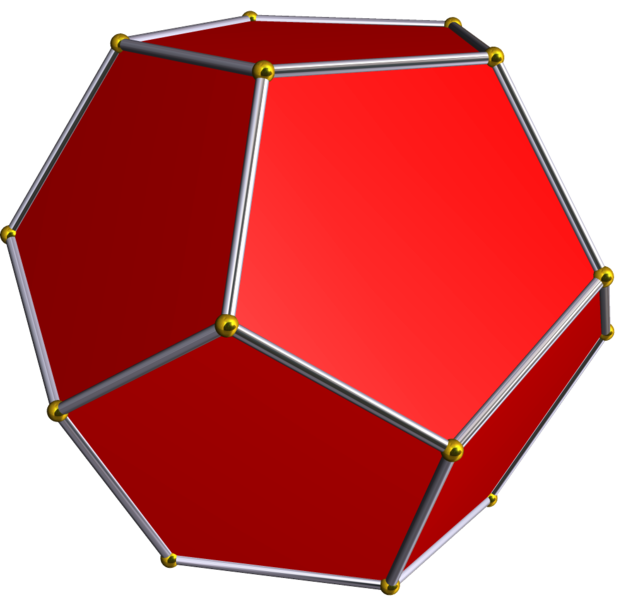
\includegraphics[width=\linewidth]{dodecahedron}
    \end{columns}
\end{frame}

\begin{frame}{``The Icosian Game''}
    \begin{center}
        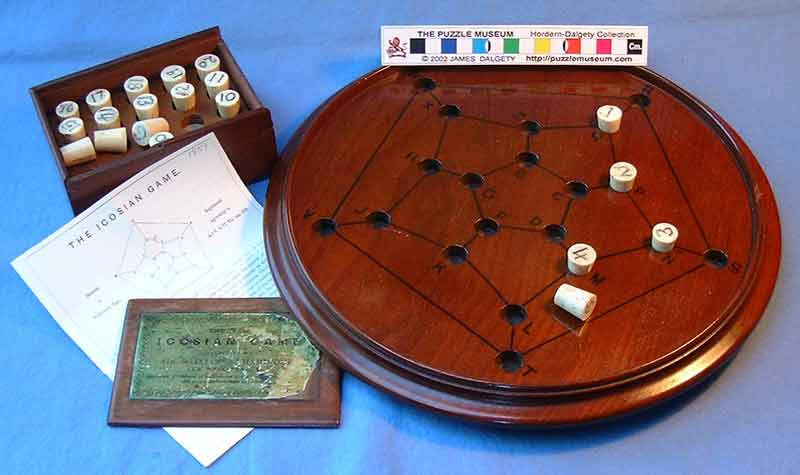
\includegraphics[width=0.9\textwidth]{icosian}

        \href{http://puzzlemuseum.com/month/picm02/200207icosian.htm}{puzzlemuseum.com}
    \end{center}
\end{frame}

\begin{frame}{Dæmi}
\begin{columns}
\column{0.5\textwidth}
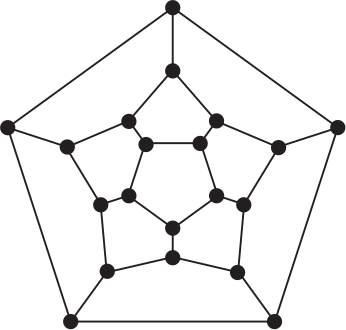
\includegraphics[width=\textwidth]{graph-hamilton}
\pause
\column{0.5\textwidth}
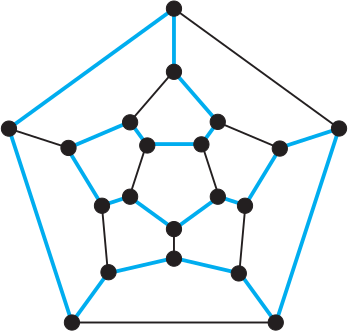
\includegraphics[width=\textwidth]{graph-hamilton-solution}
\end{columns}
\end{frame}

\begin{frame}{Hamilton- vegir og rásir}
    \begin{tcolorbox}[title=Hamilton-vegir og rásir]
        Einfaldur vegur í óstefndu neti sem fer í gegnum hvern hnút nákvæmlega einu sinni er kallaður Hamilton-vegur (e. \emph{Hamilton path}). Einföld rás sem fer nákvæmlega einu sinni í gegnum hvern hnút netsins er kölluð Hamilton-rás (e. \emph{Hamilton circuit}).
    \end{tcolorbox}
    Innihalda þessi net Hamilton-rásir? En Hamilton-vegi?
    \begin{center}
        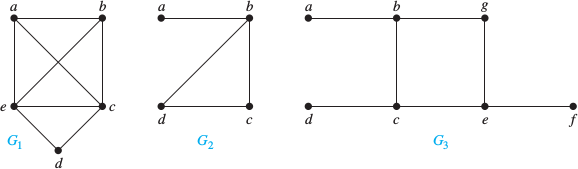
\includegraphics[width=0.8\textwidth]{graph-hamilton-examples}
    \end{center}
\end{frame}

\begin{frame}{Hagnýtingar}
    \begin{itemize}
        \item Hægt er að leysa alls kyns vandamál með því að setja þau fram sem leit að Hamilton-rás
        \begin{itemize}
            \item Frægt $NP$-complete vandamál
        \end{itemize}
        \item Praktísk dæmi
        \begin{itemize}
            \item Sorphirða, póstútburður\ldots
            \item Rafrásasmíði
        \end{itemize}
    \end{itemize}
\end{frame}

\begin{frame}{Leitin að Hamilton-rásum}
    \begin{itemize}
        \item Getum við fundið einfalda leið til að athuga hvort að gefið net innihaldi Hamilton-rás? \pause
        \begin{itemize}
            \item Engin slík leið er þekkt
        \end{itemize}
        \item Nokkur nægjanleg skilyrði eru þekkt
        \item Engin skilyrði sem eru bæði nauðsynleg og nægjanleg eru þekkt
    \end{itemize}
\end{frame}

\begin{frame}{Einfaldar staðhæfingar}
\begin{itemize}[<+->]
 \item Net sem inniheldur hnút af stigi 1 inniheldur ekki Hamilton-rás
 \item Hafi hnútur í neti stigið 2 hljóta báðir leggirnir sem snerta hnútinn að vera hluti af Hamilton-rás í netinu (sé slík til)
 \item Fullskipaða netið $K_n$ með $n \geq 3$ inniheldur Hamilton-rás
\end{itemize}
\end{frame}

\begin{frame}{Setningar}
    \begin{tcolorbox}[title=Setning Diracs]
        Sé stig allra hnúta í einföldu óstefndu neti með $n \geq 3$ hnútum a.m.k. $\frac{n}{2}$ hefur netið Hamilton-rás.
    \end{tcolorbox}
    \begin{tcolorbox}[title=Setning Ores]
        Látum $G$ vera einfalt óstefnt net með $n \geq 3$ hnúta. Gildi að $\deg(u) + \deg(v) \geq n$ fyrir sérhverja óaðlæga hnúta $u$ og $v$ í $G$, þá hefur netið Hamilton-rás.
    \end{tcolorbox}
\end{frame}

\section{Erfiðleikastig}

\begin{frame}{``Hamilton'' er NP-complete}
    \begin{itemize}
        \item Þegar Hamilton-rás hefur verið fundin er auðvelt að staðfesta hvort lausnin sé rétt
        \begin{itemize}
            \item Hins vegar virðist vera erfitt að ákvarða hvort net hefur Hamilton-rás til að byrja með
            \begin{itemize}
                \item Þá þarf að finna rásina
            \end{itemize}
            \item Nál í heysátu
        \end{itemize}
        \item Við höfum áður leitt rök að því að ``boolean satisfiability problem'' (SAT) sé erfitt vandamál
        \begin{itemize}
            \item Getum sýnt að hægt er að leysa SAT með því að setja það fram sem leit að Hamilton-rás
        \end{itemize}
    \end{itemize}
\end{frame}

\begin{frame}{Upprifjun: Og-að staðalsnið}
    Fyrir sérhverja yrðingu má finna jafngilda yrðingu á og-uðu staðalsniði (e. \emph{conjunctive normal form}):
    \[
     (b_{11} \lor b_{12} \lor \ldots \lor b_{1r_1} ) \land (b_{21} \lor b_{22} \lor \ldots \lor b_{2r_2} ) \land \ldots \land (b_{n_1} \lor b_{n_2} \lor \ldots \lor b_{nr_n} )
    \]
    
    \[
     = \bigwedge_{i=1}^n \bigvee_{j=1}^{r_n}b_{ij}
    \]
    
    Þar sem sérhvert $a_{ij}$ er á sniðinu $p$ eða $\lnot p$ fyrir yrðingabreytu $p$.
\end{frame}

\begin{frame}{Hugmyndin á bak við umbreytinguna}
    \begin{itemize}
        \item Einfölduð lýsing á aðferðinni:
        \begin{itemize}
            \item Finnum græju (e. \emph{gadget}) sem táknar hverja breytu um sig
            \item Finnum græju sem táknar klausurnar
            \item Tengjum græjurnar saman
            \item Sýnum að netið hafi Hamilton-rás þ.þ.a.a. formúlan sé uppfyllanleg
        \end{itemize}
        \item Skoðum tilbrigði - leit að stefndri Hamilton-rás í stefndu neti
    \end{itemize}
\end{frame}

\begin{frame}{Dæmi}
    Formúlan $(x \lor y) \land (\overline{x} \lor \overline{y})$
    \begin{center}
        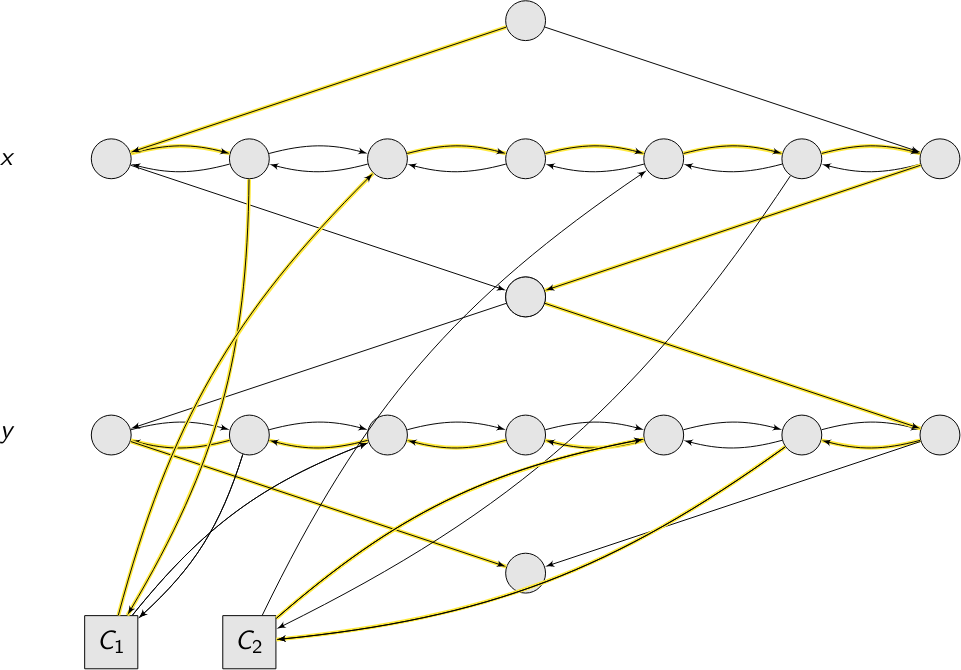
\includegraphics[width=0.95\textwidth]{hamsat}

        \tiny \url{https://www.cs.umd.edu/~gasarch/COURSES/452/F14/hamtalk.pdf}
    \end{center}
\end{frame}

\section{Leit að stystu vegum}

\begin{frame}{Vegin net}
Við getum geymt meiri upplýsingar í neti með því að ákvarða tölu fyrir hvern legg í netinu.
\begin{center}
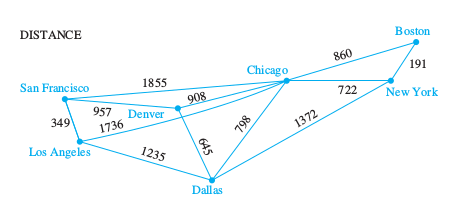
\includegraphics[width=0.7\textwidth]{graph-weighted}
\end{center}
Slíkt net er kallað vegið net (e. \emph{weighted graph}).
\end{frame}

\begin{frame}{Hagnýtingar}
\begin{itemize}
 \item Látum vegið net tákna vegakerfi þar sem þyngd leggja táknar fjarlægð milli borga
 \begin{itemize}
  \item Hver er léttasta leiðin á milli tveggja borga?
  \item Hver er léttasta leiðin sem tekur til allra borganna og endar á sama stað og hún byrjaði á?
 \end{itemize}
 \item Látum vegið net tákna rafmagnsdreifikerfi þar sem þyngd leggja táknar burðargetu rafmagnslína
 \begin{itemize}
  \item Hver er heildarburðargeta kerfisins?
  \item Hvaða kafli er mest veikburða?
 \end{itemize}
\end{itemize}
\end{frame}

\begin{frame}{Dæmi}
\begin{columns}
\column{0.6\textwidth}
Hver er léttasta leiðin á milli hnútanna $a$ og $z$?
\begin{center}
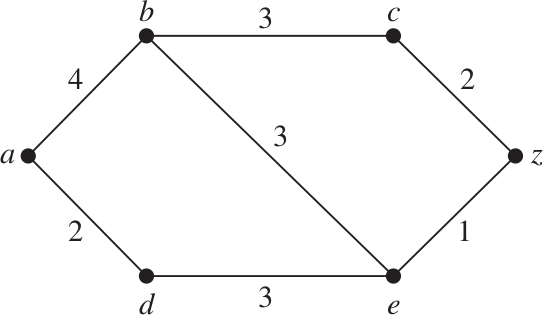
\includegraphics[width=\textwidth]{shortest-path-example}
\end{center}
\column{0.4\textwidth}
\begin{itemize}
 \item Getum leitað skipulega
 \item Finnum endurtekið léttustu leið á milli $a$ og hnúts sem við höfum ekki skoðað áður þar til við höfum fundið léttustu leið að $z$
\end{itemize}
\end{columns}
\end{frame}

\begin{frame}{Dæmi}
\begin{columns}
\column{0.6\textwidth}
Hver er léttasta leiðin á milli hnútanna $a$ og $z$?
\begin{center}
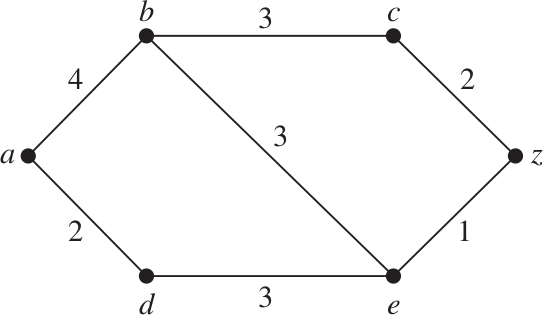
\includegraphics[width=\textwidth]{shortest-path-example}
\end{center}
\column{0.4\textwidth}
\begin{itemize}
 \item Fjarlægð 1:
 \begin{itemize}
  \item $a, d$: þyngd 2
  \item $a, b$: þyngd 4
 \end{itemize} \pause
 \item Fjarlægð 2:
 \begin{itemize}
  \item $a, b, c$: þyngd 7
  \item $a, d, e$: þyngd 5
  \item $a, b, e$: þyngd 7
 \end{itemize} \pause
 \item Fjarlægð 3:
 \begin{itemize}
  \item $a, b, c, z$: þyngd 9
  \item $a, d, e, z$: þyngd 6
 \end{itemize}
 \item Lítur út fyrir að léttasta leiðin hafi þyngd 6
\end{itemize}
\end{columns}
\end{frame}

\begin{frame}{Reiknirit Dijkstras}
\begin{center}
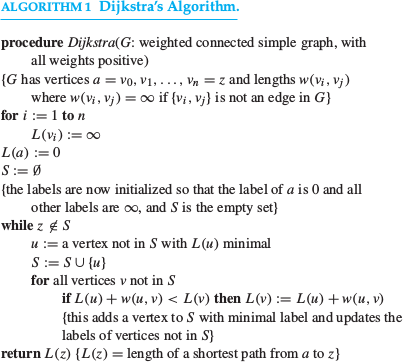
\includegraphics[width=0.8\textwidth]{dijkstras-algorithm}
\end{center}
\end{frame}

\begin{frame}{Dæmi}
    \begin{center}
        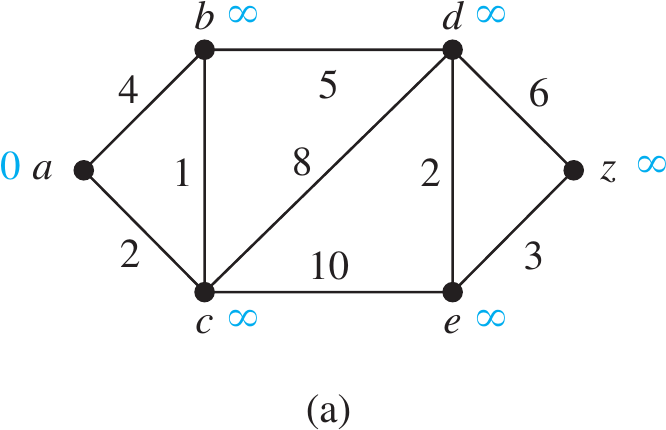
\includegraphics[width=\textwidth]{dijkstra1}
    \end{center}
\end{frame}

\begin{frame}{Dæmi}
    \begin{center}
        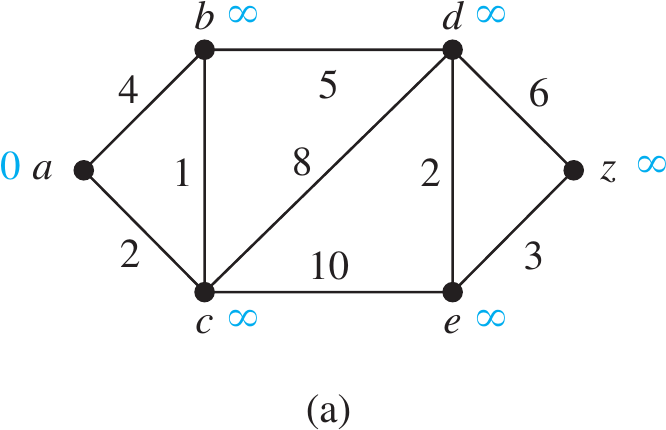
\includegraphics[width=\textwidth]{dijkstra1}
    \end{center}
\end{frame}

\begin{frame}{Dæmi}
    \begin{center}
        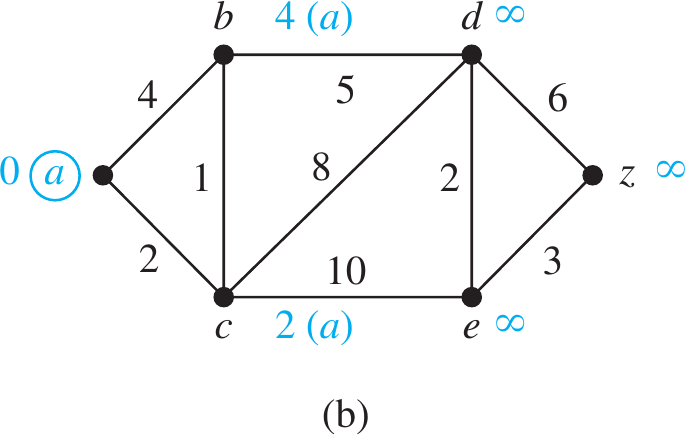
\includegraphics[width=\textwidth]{dijkstra2}
    \end{center}
\end{frame}

\begin{frame}{Dæmi}
    \begin{center}
        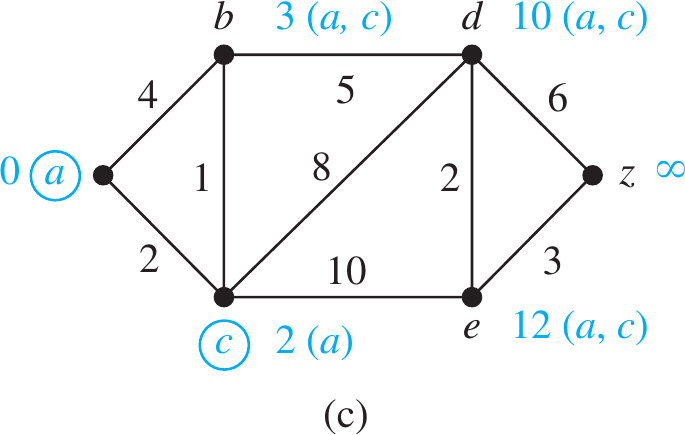
\includegraphics[width=\textwidth]{dijkstra3}
    \end{center}
\end{frame}

\begin{frame}{Dæmi}
    \begin{center}
        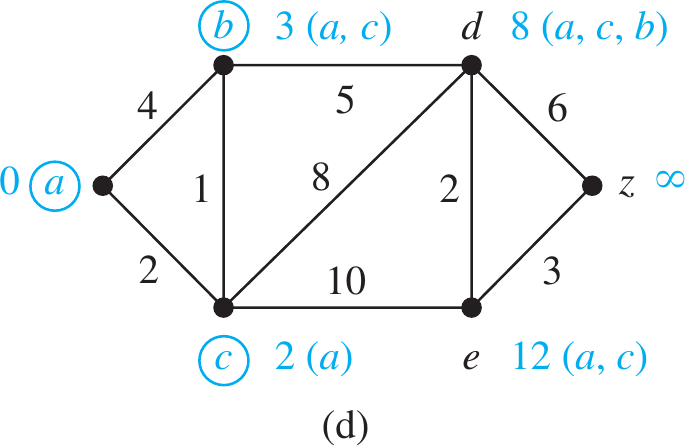
\includegraphics[width=\textwidth]{dijkstra4}
    \end{center}
\end{frame}

\begin{frame}{Dæmi}
    \begin{center}
        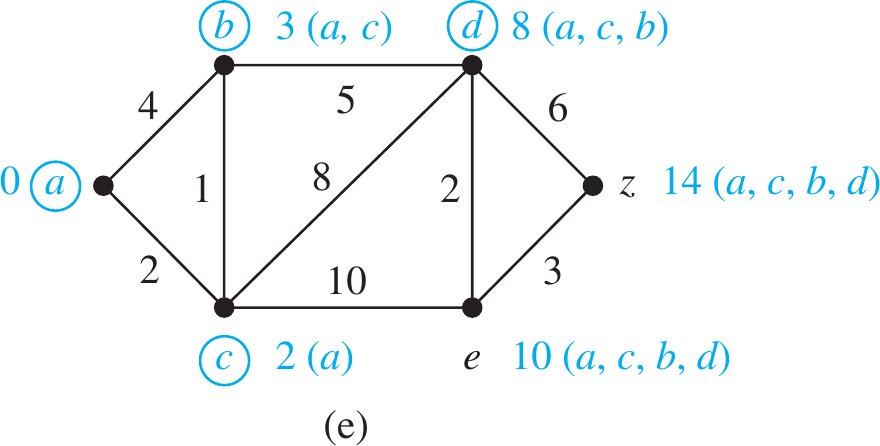
\includegraphics[width=\textwidth]{dijkstra5}
    \end{center}
\end{frame}

\begin{frame}{Dæmi}
    \begin{center}
        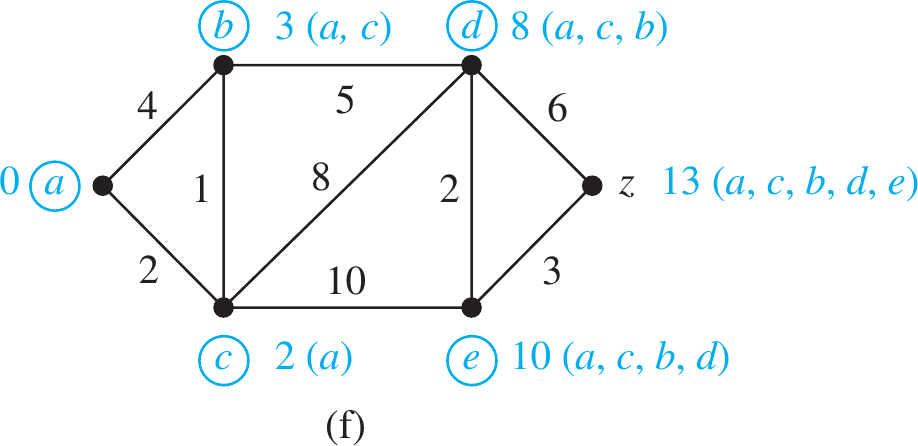
\includegraphics[width=\textwidth]{dijkstra6}
    \end{center}
\end{frame}

\begin{frame}{Dæmi}
    \begin{center}
        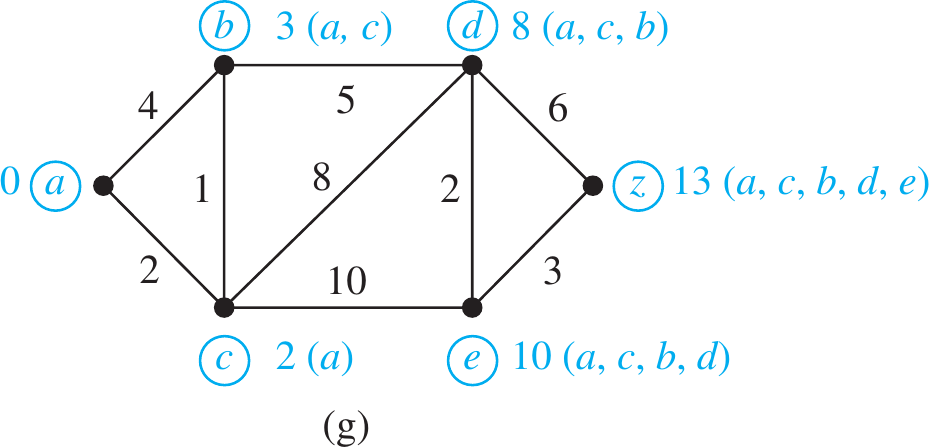
\includegraphics[width=\textwidth]{dijkstra7}
    \end{center}
\end{frame}

\begin{frame}{Dijkstra á fleti}
    \begin{itemize}
        \item Mjög algengt er að láta þyngd leggja í neti tákna fjarlægðir 
        \item Hægt er að greypa net í flöt þannig að hægt sé að nota aðferðir úr rúmfræði
        \begin{itemize}
            \item Fáum oftast Evklíðskt net (e. \emph{euclidean graph})
            \item Getum skilgreint almennari firð (e. \emph{metric})
        \end{itemize}
        \item Tölvuleikir skipta flötum oft í smærri reiti svo úr verður ``rúðustrikaður'' flötur
        \begin{itemize}
            \item Einn hnútur fyrir hverja rúðu, aðlægar rúður tengdar með legg
            \item Fjarlægðir reiknaðar með aðferðum sem eru sambærilegar við Dijkstra
            \item \href{https://qiao.github.io/PathFinding.js/visual/}{PathFinding.js}
        \end{itemize}
    \end{itemize}
\end{frame}

\section{Farandssöluvandamálið}

\begin{frame}{Farandssöluvandamálið}
    Farandssöluvandamálið (e. \emph{The Traveling Salesperson Problem} eða \texttt{TSP}) er líklega frægasta netavandamálið. Þýdd lýsing Karl Mengers frá 1930 (\href{https://homepages.cwi.nl/~lex/files/histco.pdf}{upprunaleg}):
    \begin{quote}
        Vandamál sendiboðans (því að þetta er vandamál sem allir póstburðarmenn þurfa að fást við, sem og margir ferðalangar) er það verkefni að finna stysta veg á milli endanlegs fjölda punkta þar sem fjarlægðin á milli hverra tveggja þeirra er þekkt. Vandamálið má auðvitað leysa með endanlegum fjölda tilrauna. Reglur sem leiða til færri tilrauna en fjölda umraðana punktanna eru ekki þekktar. Sú regla að fyrst skuli fara til þess punkts sem næst er, svo þess sem er þessum næsta punkti næstur o.s.frv., skilar almennt ekki stystu leið.
    \end{quote}
\end{frame}

\begin{frame}{Farandssöluvandamálið}
\begin{itemize}
 \item Nútímaframsetning: hvernig má finna er léttustu rás í óstefndu, vegnu, fullskipuðu neti sem tekur til allra hnúta? \pause
 \begin{itemize}
  \item Einfaldasta leiðin: Finna allar Hamilton-rásir í netinu til að ákvarða þá stystu
  \item Vandamál: Í fullskipuðu neti eru $(n-1)!$ möguleikar á að mynda Hamilton-rás
  \begin{itemize}
   \item Hamilton-rásir eru eins í báðar áttir, þurfum að skoða $\frac{(n-1)!}{2}$ möguleika
   \item Ekki praktískt
  \end{itemize}
 \end{itemize}
 \item Þetta vandamál er $NP$-erfitt (e. \emph{NP-hard})
 \item Í alvörunni notum við nálgunarreiknirit (e. \emph{approximation algorithms}) eða brjóstvitsaðferðir (e. \emph{heuristic algorithms})
\end{itemize}
\end{frame}

\begin{frame}{Samband mengjanna (Wikipedia)}
    \begin{center}
    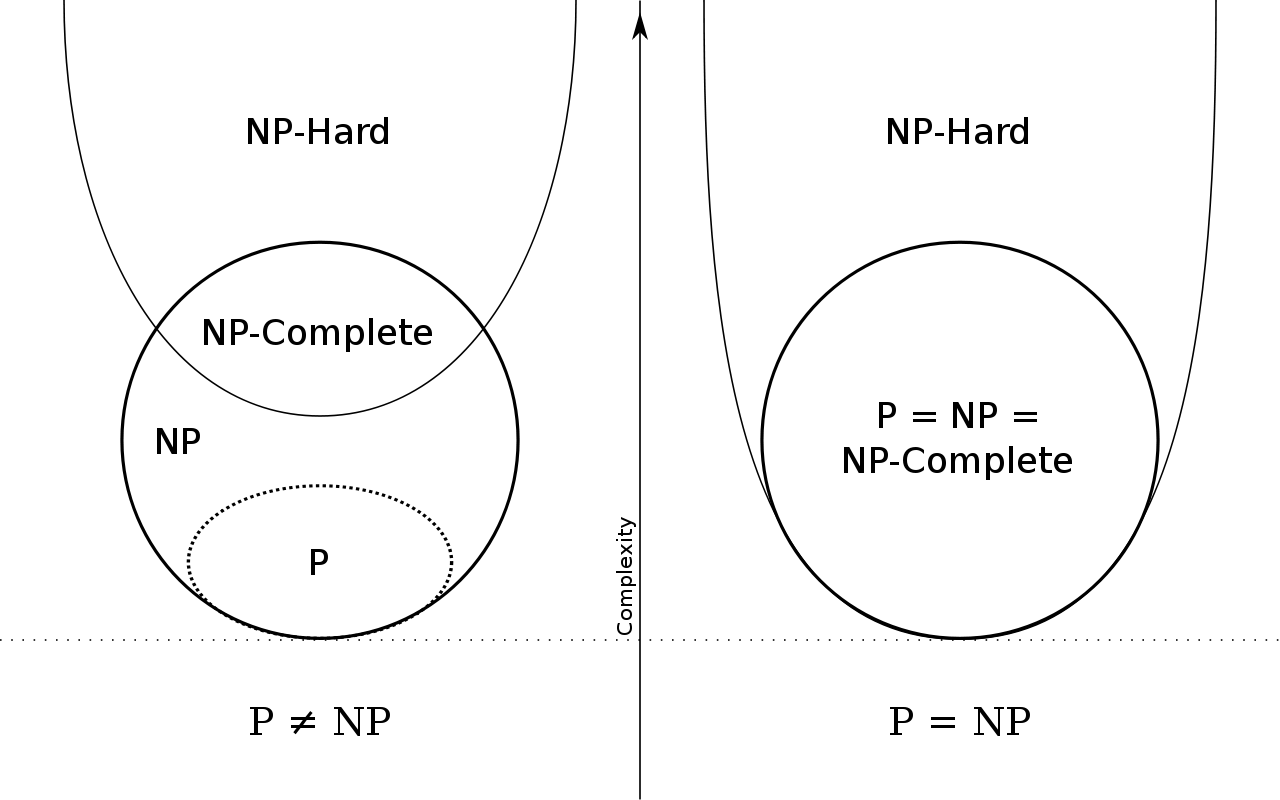
\includegraphics[width=\textwidth]{P-NP}
    \end{center}
\end{frame}


\begin{frame}{Næst}
Lagnet (kafli 10.7) og litun neta (kafli 10.8).
\end{frame}


\end{document}
